% Options for packages loaded elsewhere
\PassOptionsToPackage{unicode}{hyperref}
\PassOptionsToPackage{hyphens}{url}
%
\documentclass[
]{book}
\title{Research Data Management Workbook}
\author{Kristin Briney}
\date{2023-08-11}

\usepackage{amsmath,amssymb}
\usepackage{lmodern}
\usepackage{iftex}
\ifPDFTeX
  \usepackage[T1]{fontenc}
  \usepackage[utf8]{inputenc}
  \usepackage{textcomp} % provide euro and other symbols
\else % if luatex or xetex
  \usepackage{unicode-math}
  \defaultfontfeatures{Scale=MatchLowercase}
  \defaultfontfeatures[\rmfamily]{Ligatures=TeX,Scale=1}
\fi
% Use upquote if available, for straight quotes in verbatim environments
\IfFileExists{upquote.sty}{\usepackage{upquote}}{}
\IfFileExists{microtype.sty}{% use microtype if available
  \usepackage[]{microtype}
  \UseMicrotypeSet[protrusion]{basicmath} % disable protrusion for tt fonts
}{}
\makeatletter
\@ifundefined{KOMAClassName}{% if non-KOMA class
  \IfFileExists{parskip.sty}{%
    \usepackage{parskip}
  }{% else
    \setlength{\parindent}{0pt}
    \setlength{\parskip}{6pt plus 2pt minus 1pt}}
}{% if KOMA class
  \KOMAoptions{parskip=half}}
\makeatother
\usepackage{xcolor}
\IfFileExists{xurl.sty}{\usepackage{xurl}}{} % add URL line breaks if available
\IfFileExists{bookmark.sty}{\usepackage{bookmark}}{\usepackage{hyperref}}
\hypersetup{
  pdftitle={Research Data Management Workbook},
  pdfauthor={Kristin Briney},
  hidelinks,
  pdfcreator={LaTeX via pandoc}}
\urlstyle{same} % disable monospaced font for URLs
\usepackage{longtable,booktabs,array}
\usepackage{calc} % for calculating minipage widths
% Correct order of tables after \paragraph or \subparagraph
\usepackage{etoolbox}
\makeatletter
\patchcmd\longtable{\par}{\if@noskipsec\mbox{}\fi\par}{}{}
\makeatother
% Allow footnotes in longtable head/foot
\IfFileExists{footnotehyper.sty}{\usepackage{footnotehyper}}{\usepackage{footnote}}
\makesavenoteenv{longtable}
\usepackage{graphicx}
\makeatletter
\def\maxwidth{\ifdim\Gin@nat@width>\linewidth\linewidth\else\Gin@nat@width\fi}
\def\maxheight{\ifdim\Gin@nat@height>\textheight\textheight\else\Gin@nat@height\fi}
\makeatother
% Scale images if necessary, so that they will not overflow the page
% margins by default, and it is still possible to overwrite the defaults
% using explicit options in \includegraphics[width, height, ...]{}
\setkeys{Gin}{width=\maxwidth,height=\maxheight,keepaspectratio}
% Set default figure placement to htbp
\makeatletter
\def\fps@figure{htbp}
\makeatother
\setlength{\emergencystretch}{3em} % prevent overfull lines
\providecommand{\tightlist}{%
  \setlength{\itemsep}{0pt}\setlength{\parskip}{0pt}}
\setcounter{secnumdepth}{5}
\usepackage{booktabs}
\ifLuaTeX
  \usepackage{selnolig}  % disable illegal ligatures
\fi
\usepackage[]{natbib}
\bibliographystyle{plainnat}

\begin{document}
\maketitle

{
\setcounter{tocdepth}{1}
\tableofcontents
}
\hypertarget{about-this-book}{%
\chapter*{About this Book}\label{about-this-book}}
\addcontentsline{toc}{chapter}{About this Book}

\hypertarget{description}{%
\section*{Description}\label{description}}
\addcontentsline{toc}{section}{Description}

The Research Data Management Workbook is made up of a collection of exercises for researchers to improve their data management. The workbook contains exercises across the data lifecycle, though the range of activities is not comprehensive. Instead, exercises focus on discrete practices within data management that are structured and can be reproduced by any researcher. The book is divided into chapters by phases of the data lifecycle, with one or more exercises in each chapter. Every exercise comes with a description of its importance, notes on how to do the exercise, and the exercise instructions.

The workbook is intended as a supplement to existing data management education. If you would like to learn more about the principles of data management, please see the article by Briney, Coates, and Goben \citet{briney_foundational_2020} or read the book ``Data Management for Researchers'' \citet{briney_data_2015}.

\hypertarget{license}{%
\section*{License}\label{license}}
\addcontentsline{toc}{section}{License}

This book is available under a Creative Commons Attribution-NonCommercial (CC BY-NC) 4.0 International license

\hypertarget{the-author}{%
\section*{The Author}\label{the-author}}
\addcontentsline{toc}{section}{The Author}

Kristin Briney is the Biology \& Biological Engineering Librarian at the California Institute of Technology and author of the books \href{https://pelagicpublishing.com/products/data-management-for-researchers-briney}{``Data Management for Researchers''} (Pelagic Publishing, 2015) and, with Becky Yoose, \href{https://www.alastore.ala.org/mdpp}{``Managing Data for Patron Privacy''} (ALA Editions, 2022). She has a PhD in chemistry and an MLIS, both from the University of Wisconsin-Madison. Her research focuses on research data management, institutional data policy, and patron privacy vis-a-vis library data handling. Kristin is an advocate for the adoption of the international date standard ISO 8601 (YYYY-MM-DD) and likes to spend her free time making data visualizations out of yarn and fabric.

\hypertarget{introduction}{%
\chapter{Introduction}\label{introduction}}

\hypertarget{documentation}{%
\chapter{Documentation}\label{documentation}}

\hypertarget{lab-notebook}{%
\section{Checking Laboratory Notebooks}\label{lab-notebook}}

\textbf{\emph{Description:}} **

\textbf{\emph{Instructions:}} **

\begin{center}\rule{0.5\linewidth}{0.5pt}\end{center}

\hypertarget{readme-txt}{%
\section{README.txt}\label{readme-txt}}

\textbf{\emph{Description:}} **

\textbf{\emph{Instructions:}} **

\begin{center}\rule{0.5\linewidth}{0.5pt}\end{center}

\hypertarget{data-dictionary}{%
\section{Data Dictionary}\label{data-dictionary}}

\textbf{\emph{Description:}} **

\textbf{\emph{Instructions:}} **

\begin{center}\rule{0.5\linewidth}{0.5pt}\end{center}

\hypertarget{file-organization-and-naming}{%
\chapter{File Organization and Naming}\label{file-organization-and-naming}}

\hypertarget{file-organization}{%
\section{File Organization}\label{file-organization}}

\textbf{\emph{Description:}} **

\textbf{\emph{Instructions:}} **

\begin{center}\rule{0.5\linewidth}{0.5pt}\end{center}

\hypertarget{file-naming}{%
\section{File Naming}\label{file-naming}}

\textbf{\emph{Description:}} \emph{File naming conventions are a simple way to add order to your files and help to find them later. Rich and descriptive file names make it easier to search for files, understand at a glance what they contain, and tell related files apart.}

\begin{figure}
\centering
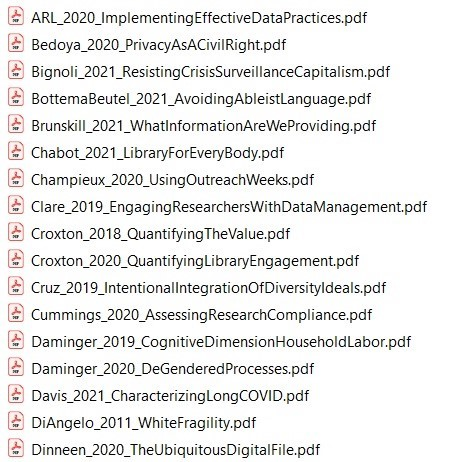
\includegraphics{images/03_FileNaming.jpg}
\caption{Screenshot of pdf's with consistent file names using the convention FirstAuthorLastName\_YEAR\_ShortTitle.pdf}
\end{figure}

\textbf{\emph{Instructions:}} \emph{This exercise guides researchers through the process of creating a file naming convention for a group of related files. Fill in each section for a group of related files following the instructions; an example for microscopy files is provided. This exercise may be redone as needed, as different groups of files require different naming conventions.}

\emph{This exercise is based on the ``File Naming Convention Worksheet'' \citet{briney_file_2020}.}

\begin{center}\rule{0.5\linewidth}{0.5pt}\end{center}

\textbf{1. What group of files will this naming convention cover?}

You can use different conventions for different file sets.

\emph{Example: This convention will apply to all of my microscopy files, from raw image through processed image.}

~

~

~

\textbf{2. What information (metadata) is important about these files and makes each file distinct?}

Ideally, pick three pieces of metadata; use no more than five. This metadata should be enough for you to visually scan the file names and easily understand what's in each one.

\emph{Example: For my images, I want to know date, sample ID, and image number for that sample on that date.}

\begin{enumerate}
\def\labelenumi{\arabic{enumi}.}
\tightlist
\item
\item
\item
\item
\item
\end{enumerate}

\textbf{3. Do you need to abbreviate any of the metadata or encode it?}

If any of the metadata from step 2 is described by lots of text, decide what shortened information to keep. If any of the metadata from step 2 has regular categories, standardize the categories and/or replace them with 2- or 3-letter codes; be sure to document these codes.

\emph{Example: Sample ID will use a code made up of: a 2-letter project abbreviation (project 1 = P1, project 2 = P2); a 3-letter species abbreviation (mouse = ``MUS'', fruit fly = ``DRS''); and 3-digit sample ID (assigned in my notebook).}

~

~

~

\textbf{4. What is the order for the metadata in the file name?}

Think about how you want to sort and search for your files to decide what metadata should appear at the beginning of the file name. If date is important, use ISO 8601-formatted dates (YYYYMMDD or YYYY-MM-DD) at the beginning of the file names so dates sort chronologically.

\emph{Example: My sample ID is most important so I will list it first, followed by date, then image number.}

\begin{enumerate}
\def\labelenumi{\arabic{enumi}.}
\tightlist
\item
\item
\item
\item
\item
\end{enumerate}

\textbf{5. What characters will you use to separate each piece of metadata in the file name?}

Many computer systems cannot handle spaces in file names. To make file names both computer- and human-readable, use dashes (-), underscores (\_), and/or capitalize the first letter of each word in the file names.

\emph{Example: I will use underscores to separate metadata and dashes between parts of my sample ID.}

~

~

~

\textbf{6. Will you need to track different versions of each file?}

You can track versions of a file by appending version information to end of the file name. Consider using a version number (e.g.~``v01'') or the version date (use ISO 8601 format: YYYYMMDD or YYYY-MM-DD).

*Example: As each image goes through my analysis workflow, I will append the version type to the end of the file name (e.g.~``\_raw'', ``\_processed'', and ``\_composite'').*

~

~

~

\textbf{7. Write down your naming convention pattern.}

Make sure the convention only uses alphanumeric characters, dashes, and underscores. Ideally, file names will be 32 characters or less.

*Example: My file naming convention is ``SA-MPL-EID\_YYYYMMDD\_\#\#\#\_status.tif'' Examples are ``P1-MUS-023\_20200229\_051\_raw.tif'' and ``P2-DRS-285\_20191031\_062\_composite.tif''.*

~

~

~

\textbf{8. Document this convention in a README.txt (or save this worksheet) and keep it with your files.}

~

~

~

\hypertarget{data-storage}{%
\chapter{Data Storage}\label{data-storage}}

\hypertarget{backups}{%
\section{Backups}\label{backups}}

\textbf{\emph{Description:}} **

\textbf{\emph{Instructions:}} **

\begin{center}\rule{0.5\linewidth}{0.5pt}\end{center}

\hypertarget{data-management-planning}{%
\chapter{Data Management Planning}\label{data-management-planning}}

\hypertarget{living-dmp}{%
\section{Living Data Management Plan}\label{living-dmp}}

\textbf{\emph{Description:}} **

\textbf{\emph{Instructions:}} **

\begin{center}\rule{0.5\linewidth}{0.5pt}\end{center}

\hypertarget{data-governance}{%
\section{Data Governance}\label{data-governance}}

\textbf{\emph{Description:}} **

\textbf{\emph{Instructions:}} **

\begin{center}\rule{0.5\linewidth}{0.5pt}\end{center}

Determine with the project PI/your collaborators:

\begin{itemize}
\tightlist
\item
  Who is allowed to reuse this data later?
\item
  Who will store the master copy of the data and for how long?
\item
  Will this data be shared publicly?
\item
  Are there security or intellectual property restrictions on the data?
\item
  Who keeps any physical research notebooks?
\end{itemize}

\hypertarget{data-sharing}{%
\chapter{Data Sharing}\label{data-sharing}}

\hypertarget{data-repository}{%
\section{Picking a Repository}\label{data-repository}}

\textbf{\emph{Description:}} **

\textbf{\emph{Instructions:}} **

\begin{center}\rule{0.5\linewidth}{0.5pt}\end{center}

\hypertarget{share-data}{%
\section{Sharing Data}\label{share-data}}

\textbf{\emph{Description:}} **

\textbf{\emph{Instructions:}} **

\begin{center}\rule{0.5\linewidth}{0.5pt}\end{center}

\hypertarget{project-wrap-up}{%
\chapter{Project Wrap Up}\label{project-wrap-up}}

\hypertarget{future-use}{%
\section{Prepare Files for Future Use}\label{future-use}}

\textbf{\emph{Description:}} **

\textbf{\emph{Instructions:}} **

\emph{This exercise has been modified from the ``Project Close Out Checklist'' \citet{briney_project_2020}.}

\begin{center}\rule{0.5\linewidth}{0.5pt}\end{center}

\textbf{Prepare Data}

Prepare data:

□ Convert data to more open/common file formats (e.g.~.CSV or .TXT)

\textbf{Record General Project Information in a \protect\hyperlink{readme-txt}{README.txt File}:}

□ Project title

□ Project description

□ Dates

□ Personnel

□ Where files are stored

□ File organization and naming conventions

\hypertarget{archive-folder}{%
\section{The Archive Folder}\label{archive-folder}}

\textbf{\emph{Description:}} \emph{To save your future-self time spent digging through all of your research files, set aside the most important files into a separate ``Archive'' folder. Do this at the end of the project while you still remember which files are important and where they are located. The Archive folder should only contain a small subset of the most important documents that are likely to be reused; you may still need to go through all of your files but, in the majority of instances, you will save time by easily finding what you need in the Archive folder.}

\textbf{\emph{Instructions:}} \emph{This exercise consists of a checklist of the key documents that are likely to be most useful in a research project archive. Create a separate folder within the larger project folder (or in a highly visible place within the storage system) labelled ``Archive''. Copy -- do not move -- the files on this checklist into the Archive folder. Add copies other important research documents, as needed. Remember, the Archive folder does not need to be comprehensive, so focus on the subset of files that are most likely to be reused or referenced in the future.}

\emph{This exercise has been modified from the ``Project Close Out Checklist'' \citet{briney_project_2020}.}

\begin{center}\rule{0.5\linewidth}{0.5pt}\end{center}

\textbf{Project Documentation}

□ README file of project information

\textbf{Data Snapshots}

□ Raw data

□ Key data analyses

□ Final data

\textbf{Code}

□ Analysis code

□ Record software version, as appropriate

\textbf{Other Research Documents}

□ Protocols

□ Survey instruments

\textbf{Research Notes}

□ Scan of research notebook

□ Digital notes

\textbf{Images}

□ Flat files of figures (e.g.~.JPG or .TIFF)

□ Editable image files (e.g.~Photoshop)

\textbf{Publications}

□ Published article in .PDF format

□ Final version of the article in editable document format (e.g.~.DOCX)

□ Posters

\textbf{Administrative Documents}

□ Grant proposals

□ Grant progress reports and final report

\hypertarget{separation}{%
\section{Separation From The Institution}\label{separation}}

\textbf{\emph{Description:}} **

\textbf{\emph{Instructions:}} **

\begin{center}\rule{0.5\linewidth}{0.5pt}\end{center}

  \bibliography{references.bib}

\end{document}
